\section{Local approximation from complete directions}\label{sec:local}

The immediate goal is an operation that enlarges one planar source
variable while retaining arbitrary passive holomorphic parameters.
Two transverse complete strip maps provide this operation; a second
construction propagates it across points not initially covered by
strips. These are the inputs to the convex approximation argument
of Section~\ref{sec:globalization}.

Write $\Delta_r=\{z\in\C:|z|<r\}$. A map on a compact set will
always mean a map holomorphic on an open neighborhood of that set.
A \emph{special pair} $D\subset D'$ consists of two closed topological
discs with piecewise smooth boundary, where $D'$ is obtained from $D$
by attaching another such disc along a proper boundary arc. All
approximation assertions use an arbitrary fixed Hermitian distance
on the target.

\begin{definition}\label{loc:property}
A complex surface $X$ has property $L$ at $x$ if there is an open
neighborhood $V$ of $x$ with the following property. For every special
pair $D\subset D'$, every pair of closed polydiscs
$P_0\Subset\operatorname{int}P\subset\C^q$, and every holomorphic map
$f$ from a neighborhood of $D\times P$ into $V$, the restriction
$f|_{D\times P_0}$ is a uniform limit of maps holomorphic near
$D'\times P_0$ with values in $X$.
The case $q=0$ is included. We call $V$ a \emph{witness neighborhood}.
\end{definition}

Witness neighborhoods can be shrunk, and the locus where $L$ holds
is consequently open.

\subsection{Planar splitting and two strip maps}

In the first strip the first coordinate is complete; in the second
strip the second coordinate is complete. Their agreement below is
along a germ of the first strip's complete central curve and a transverse
starting section of the second strip, not along both complete
central curves. This agreement will make the overlap error small
without restricting either complete direction. The conclusion is
also allowed at a displaced point on the second strip's central
curve, a feature needed later when two leaves meet tangentially.

\begin{samepage}
\begin{proposition}[Two complete directions]\label{loc:criterion}
Suppose there are holomorphic maps
\[
\sigma_1:\C\times\Delta_b\longrightarrow X,\qquad
\sigma_2:\Delta_b\times\C\longrightarrow X
\]
which are locally biholomorphic at $(0,0)$ and satisfy
$\sigma_1(z,0)=\sigma_2(z,0)$ for small $z$. If $\sigma_2$ is
locally biholomorphic at $(0,c)$, then $L$ holds at
$x=\sigma_2(0,c)$.

The same conclusion holds for a sequence of pairs whose long
coordinate domains are discs of radii tending to infinity, whose
bounded-coordinate radii are bounded below, and whose maps converge
near $(0,0)$ and, for the second map, near $(0,c)$ to the above
nondegenerate germs. Exact axis agreement is required for every pair.
In this version $x$ is the value of the limiting second germ at $(0,c)$.
\end{proposition}
\end{samepage}

To construct an extension, we will choose a polynomial map
$h=(h_1,h_2)$ on the source. On one planar piece only $h_2$ must
be small, so that the first strip can be used; on the complementary
pieces only $h_1$ must be small, so that the second strip can be
used. Both coordinates are small on their overlaps. The next lemma
arranges these pieces while keeping the original disc in one of
the second-strip pieces.

\begin{lemma}\label{loc:pieces}
Given a special pair $D\subset D'$ and an open neighborhood $N$ of
$D$, there are compact sets $A,B_0,B_1\subset\C$ and bounded open
sets $U_A,U_0,U_1$ such that
\[
\begin{gathered}
\overline{U_A}\subset\operatorname{int}A,\qquad
\overline{U_i}\subset\operatorname{int}B_i\quad(i=0,1),\\
D\subset U_0,\qquad D'\subset U_A\cup U_0\cup U_1,\\
A\cap D=\varnothing,\qquad B_0\cap B_1=\varnothing,\qquad B_0\subset N.
\end{gathered}
\]
The compact sets $D\cup A$ and $B_0\cup B_1$ are polynomially convex.
For $U_B=U_0\cup U_1$, the two closed fringes
$\overline{U_A\setminus U_B}$ and $\overline{U_B\setminus U_A}$
have positive distance.
\end{lemma}

\begin{proof}
An ambient homeomorphism of the plane takes the attached-disc pair
to $D=[-2,0]\times[-1,1]$ and $D'=[-2,3]\times[-1,1]$.
Indeed, compatible parametrizations of the attaching arc and the
remaining boundary arcs extend over both discs by
Jordan--Schoenflies; the resulting outer boundary parametrization
extends across the exterior.
In this model choose
\[
0<c<c'<a'<a<b<b'<d'<d<3,\qquad 0<\delta<\epsilon.
\]
Use the following horizontal intervals:
\[
\begin{array}{c|c|c}
&\text{compact piece}&\text{open piece}\\ \hline
B_0,\ U_0&[-2-\epsilon,a]&(-2-\delta,a')\\
A,\ U_A&[c,d]&(c',d')\\
B_1,\ U_1&[b,3+\epsilon]&(b',3+\delta).
\end{array}
\]
All compact rectangles have vertical interval
$[-1-\epsilon,1+\epsilon]$, and all open rectangles have interval
$(-1-\delta,1+\delta)$. Take $a,\epsilon$ small enough that $B_0$
is in the prescribed neighborhood. The closed fringes are disjoint
compact sets, as is seen from their horizontal intervals
$[a',b']$ and $[-2-\delta,c']\cup[d',3+\delta]$.
Pull the sets back by the homeomorphism. Compact containment and
positive separation persist. The compact unions in the statement
are unions of two disjoint filled Jordan discs, hence have connected
complement and are polynomially convex.
\end{proof}

Figure~\ref{fig:pieces} displays the complementary coordinate control
for $h=(h_1,h_2)$: the first coordinate is small on the two outer pieces,
and the second is small on the middle piece.
\begin{figure}[ht]
\centering
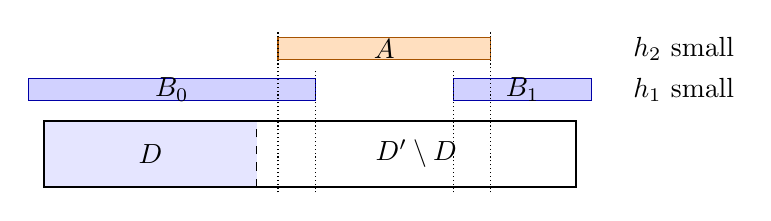
\begin{tikzpicture}[x=1.35cm,y=0.65cm]
 \fill[blue!10] (-2,-0.65) rectangle (0,0.65);
 \draw[thick] (-2,-0.65) rectangle (3,0.65);
 \draw[dashed] (0,-0.65)--(0,0.65);
 \node at (-1,0) {$D$};
 \node at (1.5,0) {$D'\setminus D$};
 \fill[blue!18] (-2.15,1.05) rectangle (0.55,1.48);
 \draw[blue!65!black] (-2.15,1.05) rectangle (0.55,1.48);
 \node at (-0.8,1.26) {$B_0$};
 \fill[blue!18] (1.85,1.05) rectangle (3.15,1.48);
 \draw[blue!65!black] (1.85,1.05) rectangle (3.15,1.48);
 \node at (2.5,1.26) {$B_1$};
 \fill[orange!25] (0.2,1.85) rectangle (2.2,2.28);
 \draw[orange!65!black] (0.2,1.85) rectangle (2.2,2.28);
 \node at (1.2,2.06) {$A$};
 \draw[densely dotted] (0.2,-0.75)--(0.2,2.4);
 \draw[densely dotted] (0.55,-0.75)--(0.55,1.65);
 \draw[densely dotted] (1.85,-0.75)--(1.85,1.65);
 \draw[densely dotted] (2.2,-0.75)--(2.2,2.4);
 \node[anchor=west] (first) at (3.45,1.26) {$h_1$ small};
 \node[anchor=west] (second) at (3.45,2.06) {$h_2$ small};
\end{tikzpicture}
\caption{Horizontal extents of the three compact pieces, shown in
separate rows. In the rectangular model, all three pieces share a vertical interval
slightly larger than that of $D'$. The two overlap bands control both
coordinates.}
\label{fig:pieces}
\end{figure}


The following is the additive Cousin splitting underlying holomorphic
spray gluing; compare \cite[Lemma~4.6]{ForstnericSplitting}.
We give its integral construction to retain bounds independent of the
number and radii of the passive parameters.

\begin{lemma}\label{loc:splitting}
Let $U_A,U_B\subset\C$ be bounded open sets with positively separated
closed fringes, and put $C=U_A\cap U_B$. For every open parameter
polydisc $P$ and every $k$, there are bounded linear operators
\[
\begin{aligned}
R_A&:H^\infty(C\times P,\C^k)\longrightarrow
H^\infty(U_A\times P,\C^k),\\
R_B&:H^\infty(C\times P,\C^k)\longrightarrow
H^\infty(U_B\times P,\C^k)
\end{aligned}
\]
satisfying $R_Au-R_Bu=u$. Their bounds depend only on the planar
sets and not on $P$ or its dimension.
\end{lemma}

\begin{proof}
Choose a smooth function $\chi$ on the plane, zero near
$\overline{U_A\setminus U_B}$ and one near
$\overline{U_B\setminus U_A}$, with bounded first derivative.
On $U_A$ extend $\chi u$ by zero off $C$; on $U_B$ extend
$(\chi-1)u$ similarly. Both extensions have planar
$\bar\partial$ derivative $u\bar\partial\chi$ on $C$ and zero
elsewhere in $\Omega=U_A\cup U_B$.
Extend this bounded coefficient by zero to $\C$ and set
\[
v(s,t)=\frac1\pi\int_C
 \frac{u(\zeta,t)\,\partial_{\bar\zeta}\chi(\zeta)}
      {s-\zeta}\,dA(\zeta).
\]
The distributional identity
$\partial_{\bar s}(1/(\pi s))=\delta_0$ gives the required
$\bar\partial$ equation. If $d$ is the diameter of $\Omega$, then
\[
\|v\|_{\Omega\times P}
\le 2d\|\bar\partial\chi\|_\infty\|u\|_{C\times P}.
\]
The kernel is locally integrable, so $v$ is continuous in $s$
and holomorphic in $t$. Thus
$R_Au=\chi u-v$ and $R_Bu=(\chi-1)u-v$ are holomorphic, have
the asserted bounds, and differ by $u$. No boundary continuity
of $u$ is needed.
\end{proof}

\begin{proof}[Proof of Proposition~\ref{loc:criterion}]
First consider complete strips. Choose $\rho>0$ so small that
$5\rho<b$, that
$\tau=\sigma_2^{-1}\circ\sigma_1$ is defined near
$\overline{\Delta}_{3\rho}^2$ using the inverse branch at the origin,
and that $D\tau$ is invertible there. Exact axis agreement gives
$\tau(z,0)=(z,0)$. The matrices $T_0(z)=D\tau(z,0)$ and their
inverses are bounded on $|z|\le2\rho$.
Choose a biholomorphic $\sigma_2$ chart $Q_c$ about $(0,c)$ whose
first coordinate has modulus less than $\rho/16$, and take a
relatively compact smaller image $V$ as the witness neighborhood.

Fix input data as in Definition~\ref{loc:property}. Choose an open
polydisc $P_*$ with
$P_0\Subset P_*\Subset\operatorname{int}P$.
In the chart $Q_c$ write $g=\sigma_2^{-1}\circ f=(g_1,g_2)$.
There is a planar neighborhood $N$ of $D$ where $g$ is defined for
parameters in a neighborhood of $\overline P_*$ and
$|g_1|<\rho/8$. No smallness of $g_2-c$ beyond membership in $Q_c$
is used in the overlap calculation.

Choose the pieces of Lemma~\ref{loc:pieces}. Products of polynomially
convex compact sets are polynomially convex. Scalar Oka--Weil
approximation therefore gives a polynomial $h_1$ in the planar and
parameter variables approximating $g_1$ on
$B_0\times\overline P_*$ and zero on $B_1\times\overline P_*$.
Its error $\epsilon_1$ can be arbitrarily small; in particular,
$|h_1|<\rho/2$ on their union. Independently, for every sufficiently
small $\eta>0$ there is a polynomial $h_2$ satisfying
\[
\|h_2-g_2\|_{D\times\overline P_*}<\eta,\qquad
\|h_2\|_{A\times\overline P_*}<\eta.
\]
Let $h=(h_1,h_2)$ and $C=U_A\cap U_B$. On $U_B\times P_*$,
$T=T_0(h_1)$ is holomorphic and boundedly invertible.
We seek corrections satisfying
\[
\tau(h+\alpha)=h+\beta,\qquad
\alpha=R_Au,\quad\beta=T R_Bu.
\]
By Lemma~\ref{loc:splitting}, this is the fixed-point equation
\[
u=\mathcal T(u):=
R_Au+T^{-1}\bigl(h-\tau(h+R_Au)\bigr)
\]
in $H^\infty(C\times P_*,\C^2)$.

On the overlap $|h_1|<\rho/2$ and $|h_2|<\eta$.
Bounded first and second derivatives of $\tau$, and its exact
axis identity, give a constant $M\ge1$ with
\[
\|T\|,\|T^{-1}\|\le M,\quad
\|\tau(h)-h\|\le M\eta,\quad
\|D\tau(h+\alpha)-T\|\le M(\eta+\|\alpha\|).
\]
These constants do not depend on the degrees or uncontrolled
coordinates of the polynomials. If $\kappa\ge1$ bounds both
splitting operators and $L_0=2M^2+1$, then on $\|u\|\le L_0\eta$,
\[
\|\mathcal T(0)\|\le M^2\eta,\qquad
\|D\mathcal T(u)\|\le
M^2\kappa(1+\kappa L_0)\eta.
\]
For small $\eta$ the last bound is at most $1/2$, the ball maps
strictly into itself, and all transition evaluations remain in
$\Delta_{3\rho}^2$. The contraction theorem gives
\[
\|\alpha\|\le\kappa L_0\eta,\qquad
\|\beta\|\le M\kappa L_0\eta.
\]

On $U_A\times P_*$ only the second coordinate of $h+\alpha$ has
to be small, and on $U_B\times P_*$ only the first coordinate
of $h+\beta$ has to be small. Consequently
$\sigma_1(h+\alpha)$ and $\sigma_2(h+\beta)$ are defined on
these full domains and agree on their overlap. On $D\times P_*$,
the second formula is evaluated close to $g$ in $Q_c$ and
approximates $f$ as $\epsilon_1,\eta\to0$. Since the union of the
planar domains contains $D'$ and $P_0\Subset P_*$, this proves $L$.

For the finite-length version choose $V$, $g$, and the two
polynomials using the limiting chart at $(0,c)$. Convergence on
slightly larger compact coordinate neighborhoods gives uniform
first and second derivative bounds, uniform inverse-chart domains,
and thus uniform constants in the contraction argument.
Exact axis agreement gives the same $O(\eta)$ initial error for
every pair. The polynomials are bounded on the fixed bounded
planar pieces and $\overline P_*$, so only a finite range of either
long coordinate is used. Choose a sufficiently late pair to contain
these ranges and make its chart near $(0,c)$ sufficiently close to
the limiting chart. The construction then approximates the original
data with the requested accuracy.
\end{proof}

\begin{remark}\label{loc:alignment}
Two strip maps locally biholomorphic at chosen meeting preimages,
with transverse central curves there, can be put in the form of
Proposition~\ref{loc:criterion}. Locally lift the
first central curve through the inverse of the second strip, writing
the lift as $(a(z),t(z))$, where its bounded coordinate is $a$.
Replace the second strip by
$\widetilde\sigma_2(z,w)=\sigma_2(a(z),t(z)+w)$.
Transversality says $a'(0)\ne0$, and time zero gives exact axis
agreement. If the original second central curve also passes through
$x$ and its strip is regular there, some finite $c$ gives a regular
chart $\widetilde\sigma_2(0,c)=x$.
For finite-length families whose central germs converge to transverse
germs through a common point, the implicit function theorem first
gives nearby intersection points and meeting preimages. Translate
the preimages to the origin and apply the same construction.
Convergence and transversality give a uniformly positive
bounded-coordinate radius; the translations and the function $t$
lose only a bounded amount of long-coordinate length. Thus this
construction also supplies the aligned families in the finite-length
part of the proposition.
\end{remark}

\subsection{Sprays, deformation, and planar gluing}

The strip criterion provides approximation when all input values lie
in one witness neighborhood. To apply it successively to a map whose
image meets several such neighborhoods, we need coordinates around
the graph of the map and a way to join close maps in those coordinates.
The next three lemmas supply exactly these tools. The use of sprays
and their gluing follows the framework of Gromov \cite{GromovOka}
and Forstneri\v c \cite{Forstneric}; here the sprays are constructed
only near the graph on a relatively compact Stein source.

\begin{lemma}[Local chart sprays]\label{loc:spray}
Let $f:S\to X$ be holomorphic on a Stein manifold, let
$K\Subset S$ be compact, and assume $f^*TX$ is holomorphically
trivial on $S$. After shrinking the source neighborhood there
is a holomorphic map $f^\sharp(z,v)$ for $z$ near $K$ and
$v\in\Delta_r^2$, with $f^\sharp(z,0)=f(z)$, such that
$v\mapsto f^\sharp(z,v)$ is injective with invertible differential.
The hypothesis on $f^*TX$ holds for a contractible Stein source
and for a planar domain times a polydisc.
\end{lemma}

\begin{proof}
The graph of $f$ is a closed Stein submanifold of $S\times X$ and
has a Stein neighborhood by the Stein neighborhood theorem
\cite{Siu}. On that neighborhood consider the vertical tangent
bundle for projection to $S$. A holomorphic frame along the graph
extends to holomorphic vertical vector fields by Cartan's
Theorem~B. Compose their small-time flows. The resulting map has
the prescribed value and a frame as its vertical differential
at $v=0$. Compactness and the holomorphic inverse function theorem
give a common radius on a neighborhood of $K$ and injectivity
in each parameter fiber.
For the last assertion, a planar domain has the homotopy type of
a one-dimensional CW complex, so every complex vector bundle on
its product with a polydisc is topologically trivial. The
Oka--Grauert principle makes it holomorphically trivial.
The same argument applies to a contractible Stein source
\cite{Forstneric}.
\end{proof}

\begin{lemma}[Deforming a map on a relatively compact Stein domain]
\label{loc:deformation}
Let $\pi:\mathcal X\to B$ be a holomorphic family, and let
$f:S\to\mathcal X_{b_0}$ be holomorphic from a Stein manifold
with image in the submersion locus of $\pi$. On every relatively
compact source domain there is a holomorphic family of maps
$f_b$ into $\mathcal X_b$ for $b$ near $b_0$, with $f_{b_0}=f$.
\end{lemma}

\begin{proof}
Work in local coordinates on $B$ at $b_0$. The graph of $f$ has
a Stein neighborhood in $S$ times the submersion locus. On this
neighborhood the surjection from tangent vectors vertical over $S$
to the pulled-back base tangent bundle admits holomorphic lifts of
the base coordinate vector fields: its kernel is coherent, and
Cartan's Theorem~B gives surjectivity on global sections. Flow the
lifts successively for the small coordinate displacements of $b$.
On a relatively compact source set a common time radius is
available. The flows are vertical over $S$, and their projections
to $B$ are the desired coordinate translations. Their composition
is the required family of maps.
\end{proof}

\begin{lemma}[Planar spray gluing]\label{loc:gluing}
Suppose two holomorphic sprays over bounded planar domains $U_A,U_B$ and
a parameter polydisc are uniformly close on their overlap, with
a positive margin in an auxiliary spray polydisc. Suppose the
first spray is a chart spray there with uniform inverse-chart
margins, and the closed planar fringes
are positively separated. If the closeness is sufficiently small,
their central maps can be glued after arbitrarily small
holomorphic corrections in the auxiliary variables. The glued
map is arbitrarily close to the first central map on any prescribed
compact subset of its domain on which that spray is fixed, or has
a uniform modulus of continuity in its auxiliary variables.
\end{lemma}

\begin{proof}
Write the sprays as $F_A$ and $F_B$. Compact chart margins give
the transition
$\gamma(s,t,v)=F_A(s,t,\cdot)^{-1}(F_B(s,t,v))
=v+E(s,t,v)$ on the overlap, with both
$\|E\|$ and $\|D_vE\|$ small on a smaller auxiliary polydisc.
The derivative estimate follows from the original closeness by
Cauchy estimates on the larger polydisc. Equality of the resulting
maps asks for $a=\gamma(b)$.
Use $a=R_Au$, $b=R_Bu$. Then
\[
u=E(s,t,R_Bu)
\]
is a contraction on a small ball in the overlap $H^\infty$ space.
Lemma~\ref{loc:splitting} supplies its uniform bounds and preserves
holomorphic dependence on the passive parameters. The resulting
corrections remain in the auxiliary polydisc and are as small
as the original mismatch. Uniform continuity on the prescribed
compact sets gives the asserted approximation.
\end{proof}

The domains in this lemma may be thin neighborhoods of compact
planar sets. In applications below the cutoff is chosen first on
a fixed overlap band. Its derivative bound, and the diameter bound
in Lemma~\ref{loc:splitting}, do not increase when the domains are
subsequently narrowed away from that band.

\subsection{One planar enlargement with passive parameters}

\begin{proposition}\label{loc:planar}
Let $K$ be a closed circular disc of radius $r$, or a closed
circular annulus with outer radius $r$, and let $f$ be holomorphic
near $K\times P$, where $P$ is a closed polydisc. Suppose that for
every $\zeta$ on the outer circle there is a coordinate witness
neighborhood $V_\zeta$ for $L$ containing $f(\{\zeta\}\times P)$.
For every $R>r$ and $P_0\Subset\operatorname{int}P$, one can
approximate $f$ uniformly on $K\times P_0$ by a map holomorphic
near the enlarged disc, respectively annulus with the same inner
radius and outer radius $R$, times $P_0$.
\end{proposition}

\begin{proof}
We give a finite construction with explicit approximation margins.
Choose a compact intermediate parameter polydisc strictly between
$P_0$ and $P$. Compactness gives a partition of the outer circle
into finitely many closed arcs, with endpoint margins, such that
all values over each slightly enlarged arc and the intermediate
parameter set lie in one coordinate witness neighborhood $V_j$.
At the common endpoint of consecutive arcs the compact set of
values lies in $V_j\cap V_{j+1}$ with a positive target margin.
Take a slightly larger outer radius than $R$ during the construction.

\emph{Attach radial spokes.}
At each endpoint choose a small filled polar rectangle crossing
the old outer circle, on which $f$ and a chart spray from
Lemma~\ref{loc:spray} have their values in both adjacent target
charts. The rectangles can be chosen mutually disjoint. Attach
to each rectangle a radial segment reaching the larger outer
radius. In one of its target charts, continue the coordinate
spray constantly along the segment from its attachment point on
the outer edge of the rectangle. This defines continuous
coordinate functions on the filled rectangle and attached segment,
holomorphic on its interior and holomorphic in the passive and
auxiliary parameters.

The planar compact set has connected complement. Mergelyan
approximation, with parameters, approximates these coordinate
functions by polynomials. Here the parameter assertion follows
directly by taking finite Taylor sums on a slightly larger
parameter polydisc and applying scalar Mergelyan to their
coefficients. Consequently the approximation can be made uniform
with an auxiliary-parameter margin, and Cauchy estimates preserve
the required spray derivatives. On the radial segment its values
remain close to the endpoint values for all parameters. A thin
neighborhood of each segment therefore also has its values in
both adjacent $V_j$'s.

Glue this extension to the old chart spray across a radial band
inside each original rectangle, using Lemma~\ref{loc:gluing}.
More explicitly, cut the union domain at a radius slightly larger
than $r$, still inside the old map domain. At the cut it consists
only of the disjoint rectangles. A radial cutoff with a fixed
transition width gives separated fringes and a bounded splitting
constant. The tubes around the longer portions of the spokes may
then be narrowed without changing that constant. Gluing errors
can be as small as desired. This produces a map near $K$ and all
spokes, close to $f$ on $K$, with all spoke values still in the
two adjacent target charts.

\emph{Fill the sectors.}
List the finitely many closed polar sectors between successive
spokes. At a given step let $K_{\rm old}$ be the union of the
original compact set, all spokes, and the sectors already filled.
The next sector $S$ meets $K_{\rm old}$ exactly on its bottom
arc and its two radial sides. Along these three sides all map
values, with a parameter margin, belong to the chosen $V_j$.
This is true initially by the spoke construction, and it remains
true after each sufficiently accurate gluing, because the sides
of every unfilled sector already belong to $K_{\rm old}$.

Choose a thin closed U-shaped band $D$ about these three sides,
inside the current map domain, and a slightly enlarged filled
sector $D'$ containing $S$ in its interior, so that $D\subset D'$
is a special pair. To see this elementary geometry, straighten
the sector to a rectangle: $D$ is a thick band around its bottom
and two side edges, and the missing central rectangle attaches
along the U-shaped portion of its boundary. The bands and
protrusions can be made as thin as needed.
All values near $D$ lie in $V_j$. Apply $L$ to the restriction
of a chart spray over the current map, regarding its small
auxiliary variables as additional passive parameters. After any
prescribed small parameter loss this gives a spray on $D'$,
arbitrarily close to the old spray on $D$.

We spell out the overlap used to glue. Fix an open band
$W\Subset\operatorname{int}D$ containing $K_{\rm old}\cap S$.
Using a slightly smaller band first, the compact remainders on
opposite sides are positively separated. A smooth cutoff can
therefore be zero near $K_{\rm old}\setminus W$ and one near
$S\setminus W$. On a sufficiently thin neighborhood of
$K_{\rm old}\cup S$, its sublevel and superlevel sets give two
open domains with separated fringes and overlap contained in $W$.
They may be chosen so that any point of $K_{\rm old}$ in the new
side also lies in the approximation band. The old spray is
defined on the first domain, the approximating spray on the
second, and they are close on their overlap with an auxiliary
margin. Lemma~\ref{loc:gluing} produces the required new map,
close to the old map on all of $K_{\rm old}$.

There are only finitely many spokes and sectors. Fix in advance
a finite nested sequence of parameter polydiscs between the
intermediate one and $P_0$. At each step choose errors smaller
than the remaining compact target-chart margins and allocate a
summable finite part of the requested final error. These choices
preserve every unfilled sector's joining sides. No chart condition
on the outer boundary of a newly filled sector is required.
At the end we have a map on a neighborhood of the desired
enlarged compact set times $P_0$, with the stated approximation.
\end{proof}

\begin{corollary}[Propagation across a small disc]\label{loc:disc}
Suppose a coordinate neighborhood contains a closed affine
complex-line disc centered at $x$, with its boundary in the open
locus where $L$ holds. Then $L$ holds at $x$.
In particular, if the complement of that locus is contained
locally in a proper analytic subset, $L$ holds everywhere.
\end{corollary}

\begin{proof}
Slightly tilt the line in two different directions through $x$.
Openness and compactness of the original boundary imply that the
two tilted discs still have boundary in the good locus, and their
tangent directions at $x$ are transverse. Thicken each disc in a
complementary coordinate by a sufficiently small fixed parameter
disc. At every boundary point the values for all parameters then
lie in one witness neighborhood; finitely many boundary patches
give one common positive transverse radius.

For each integer $n$, apply Proposition~\ref{loc:planar} once to
each thickened disc, enlarging its long coordinate to radius
$n$, retaining a fixed smaller transverse radius, and making its
error on the initial product less than $1/n$. The resulting
finite strips converge near their centers to the original
coordinate charts. Their limiting long directions are transverse.
Remark~\ref{loc:alignment} and the finite-length case of
Proposition~\ref{loc:criterion} imply $L$ at $x$.

If a proper analytic subset $E$ contains the exceptional points
in a coordinate neighborhood of $x$, choose a complex line
through $x$ not contained in $E$. Its intersection with $E$ is
discrete near $x$, so a sufficiently small circle on that line
avoids $E$. The first assertion applies.
\end{proof}

\begin{remark}
The proof also records a useful uniform version: finitely many
coordinate discs whose boundaries lie in fixed compact subsets of
the good locus retain the required boundary containment after
sufficiently small deformations of the coordinate charts.
All arguments in this section concern one planar variable with
passive parameters. No approximation theorem for arbitrary
multidimensional source compacta has been used.
\end{remark}
